\documentclass[letterpaper,12pt]{article}

\usepackage[top=1in, left=1.25in, right=1.25in, bottom=1in]{geometry}
\usepackage[utf8]{inputenc}
\usepackage[T1]{fontenc}
\usepackage[spanish]{babel}
\usepackage{graphicx}
\usepackage{float}
\usepackage[backend=biber,style=numeric,sorting=none]{biblatex}
\addbibresource{bib/referencias.bib}

\begin{document}

\tableofcontents
\clearpage

\section{Introducción}

\begin{itemize}
\item \textbf{Planteamiento del Problema:} Crear solución a la serie de problemas propuestos, y utilizar funciones recursivas para dicha solución.
\item \textbf{Motivación:} Consideramos que es importante el realizar esta práctica para fortalecer las bases de la programación en Java, mediante la implementación de funciones recursivas para resolución de factorial, serie de Fibonacci y conjetura de Collatz, así mismo la correcta estructuración para un menú de opciones.
\item \textbf{Objetivos:} Aprender a realizar funciones recursivas y un menú de opciones en Java.
\end{itemize}
\section{Marco Teórico}
\textbf{Factorial:} Es el producto de todos los números enteros positivos desde 1 hasta ese número n. Su representación matemática es: n! = n * (n-1)! ~\cite{factorial}


\textbf{Serie de Fibonacci:} Es una serie de números en la que cada número es una suma de los dos anteriores, empezando siempre ésta en 0 y 1 y terminando en n. Su representación matemática es: F(n) = F(n-1) + F(n-2).~\cite{fibonacci}


\textbf{Conjetura de Collatz:} Es un algoritmo que asegura que todo número entero positivo siempre llegara a 1 mediante la recursión de dos casos, su representación matemática es: f(n) = n/2 si n es par ; 3n + 1 si n es impar~\cite{collatz}

\section{Desarrollo}

\textbf{Solución teórica de los ejercicios:}

Para los tres ejercicios realizados en clase, empezamos planteando la parte teórica, buscando el caso base y después la operación que va a permitir que la fución realice lo requerido y de forma recursiva. 
\begin{enumerate}

    \item \textbf{Factorial}

    El caso base del factorial, es cuando \textbf{n} es igual a \textbf{1}, la fórmula del factorial es \textbf{n(n-1)}, entonces en el código, se rompe la recursividad cuando el número es igual a 1, y cuando no lo es, se regresa el número multiplicado por la misma función factorial pero disminuido en 1.

    \item \textbf{Serie de Fibonacci}

    En fibonacci los casos base son cuando \textbf{n} es igual a \textbf{0} ó \textbf{1}. Para que la función haga lo que queremos, necesitamos sumar el numero anterior con el número anterior a ese hasta llegar al caso base, y es lo que hacemos en el código, si no se rompe la recursividad, se hace la suma de los dos números anteriores hasta que la recursividad se rompa.  

    \clearpage

    \item \textbf{Conjetura de Collatz}

    En la Conjetura de Collatz se realiza una evaluación dentro de la función para determinar si es par o impar y realizar su correspondiente operación; si \textbf{n} es par se divide entre 2 \textbf{(n/2)} y se llama de nuevo a la función de forma recursiva, en caso de ser \textbf{n} impar se multiplica por 3 y se suma 1 \textbf{(n*3+1)}, pero siempre evaluando si se llegó al caso base; el caso base es llegar al \textbf{1}, pero anteriormente a este número entra al ciclo infinito del \textbf{4,2,1,4,2,1...}, por ello es necesario cerrar ese ciclo con el \textbf{1}. 
    
\end{enumerate}




\section{Resultados}

\begin{figure}[H]
    \centering
    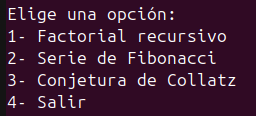
\includegraphics[width=12cm]{Imagenes/Menu.png}
    \caption{Todas las funciones integradas en un solo menú}
\end{figure}

\begin{figure}[H]
    \centering
    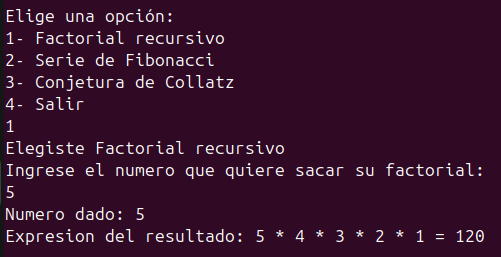
\includegraphics[width=15cm]{Imagenes/Factorial.png}
    \caption{\centering Opción 1, mostrando el factorial de un número ingresado y la operación que se realizo}
\end{figure}

\begin{figure}[H]
    \centering
    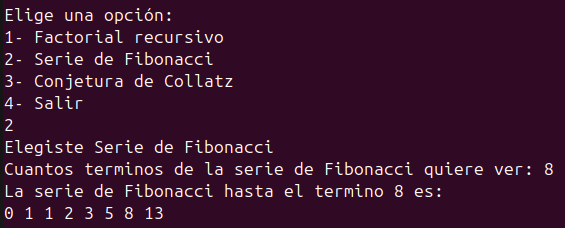
\includegraphics[width=15cm]{Imagenes/Fibonacci.png}
    \caption{\centering Opción 2, mostrando la serie de Fibonacci con los términos que el usuario solicito}
\end{figure}

\begin{figure}[H]
    \centering
    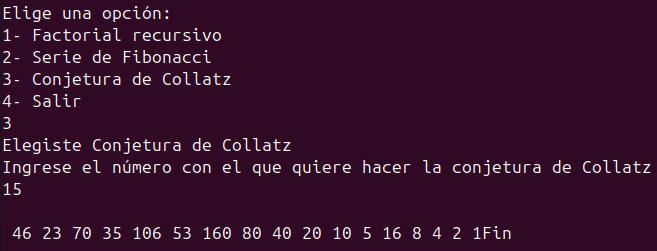
\includegraphics[width=15cm]{Imagenes/Collatz.png}
    \caption{\centering Opción 3, mostrando inmediatamente los resultados de las operaciones que realiza la conjetura}
\end{figure}

\section{Conclusiones}


La implementación del menú de opciones en Java permitió aplicar los conceptos teóricos vistos en clase mediante la resolución del factorial recursivo, la serie de Fibonacci y la conjetura de Collatz. Los objetivos de la práctica se cumplieron al desarrollar un menú con las funciones recursivas funcionales.

\clearpage

\printbibliography

\clearpage

\section{Reto para token}
El triángulo de Pascal es una matriz de forma triangular, la cuál en cada una de sus filas empiezan y terminan en uno, y los dígitos son la suma de los dos dígitos encima de él.

Para manejar el triángulo de pascal en código, nos ayudamos usando el triángulo con 2 posiciones, una que mida las filas o pisos, y otra que mida las posiciones dentro del triángulo.

\begin{figure}[H]
    \centering
    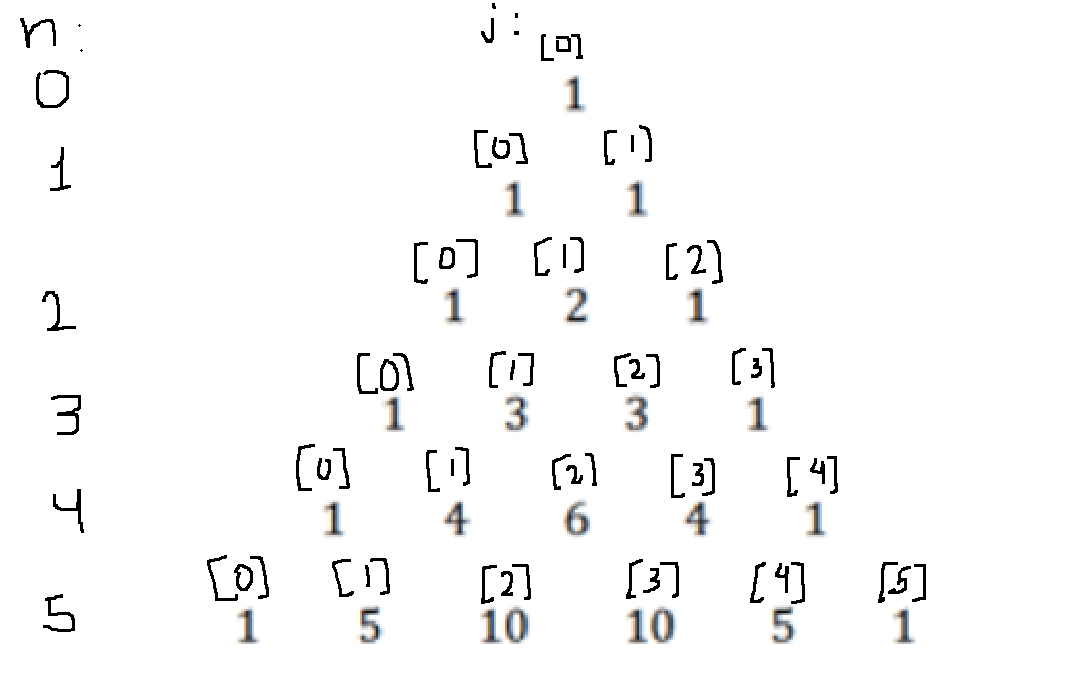
\includegraphics[width=15cm]{Imagenes/ejemplo.png}
    \caption{\centering Forma gráfica de entender el código del Triángulo de Pascal}
\end{figure}

El caso base del triángulo de pascal es cuando llegamos a los bordes del triángulo, donde en esos casos siempre es uno, y si no se cumple el caso base, se hace la suma de la posición de \textbf{(n-1, j-1)} y \textbf{(n-1, j)}, lo que significa que hace la suma de los dos números que están en el piso de arriba justo encima del número a calcular.

\clearpage

Usamos una función recursiva, y lo que hace es calcular el número en la posición de \textbf{n} y \textbf{j} que es ingresada, usando la lógica explicada anteriormente, y para que se imprima la pirámide completa, usamos 2 ciclos \textbf{for} anidados que van iterando en las posiciones de la pirámide y calculando todos los números.

Usamos otro ciclo \textbf{for} que va imprimiendo espacios según el nivel en el que está para que la pirámide sí tenga forma de pirámide.

\begin{figure}[H]
    \centering
    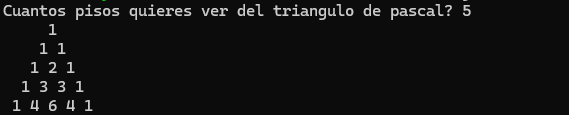
\includegraphics[width=15cm]{Imagenes/pascal.png}
    \caption{\centering Código ejecutado}
\end{figure}

\end{document}